%==============================================================================
\documentclass[MathematicsNumericsDerivationsAndOpenFOAM.tex]{subfiles}
\begin{document}
%==============================================================================


\section{The Conserved Momentum Equation}
\label{SECTION::momentum}
%
%
	The following section discusses the derivation of the momentum equation
    which is also named the Navier-Stokes equation.

	The derivation of the conserved momentum equation is similar to the
    continuity equation. Again, we will use the volume element d$V$. The main
    difference in the momentum equation compared to the mass conservation
    equation is as follows: The quantity of the momentum is a vector and
    not a scalar. Thus, the momentum is not only transported/advected via the
    flux through the surfaces of the volume element.
%
%
	In general, we are allowed to define the momentum transport and its change
    inside the volume d$V$ as follow:
%
%
\begin{equation}
\left[
 \vphantom{\begin{matrix} . \\ . \\ . \\ . \end{matrix}}
 \begin{matrix}
  \rmm{rate~of}\\
  \rmm{momentum}\\
  \rmm{accumulation}
 \end{matrix}
\right]
=
\left[
 \begin{matrix}
  \rmm{rate~of}\\
  \rmm{momentum}\\
  \rmm{entering~the}\\
  \rmm{volume}
 \end{matrix}
\right]
-
\left[
 \begin{matrix}
  \rmm{rate~of}\\
  \rmm{momentum}\\
  \rmm{leaving~the}\\
  \rmm{volume}
 \end{matrix}
\right]
+
\left[
 \vphantom{\begin{matrix} . \\ . \\ . \\ . \end{matrix}}
 \begin{matrix}
  \rmm{sum~of~forces}\\
  \rmm{that~act~on}\\
  \rmm{the~volume}
 \end{matrix}
\right] .
\label{EQUATION::momentum}
\end{equation}
%
%
	Figure \ref{Abb_Grundlagen_2_Impulserhaltung} shows the same volume element
    as given in figure \ref{figure::massFigure}, but now including another
    transport phenomenon that acts on the surfaces (only the $x$ direction is
    presented). This transport of the momentum is based on molecular effects.
    The molecular transport acts always normal and tangential to the surface
    and is an outcome or property of the vector quantity.
%
%
%
%
\begin{figure}[!b]
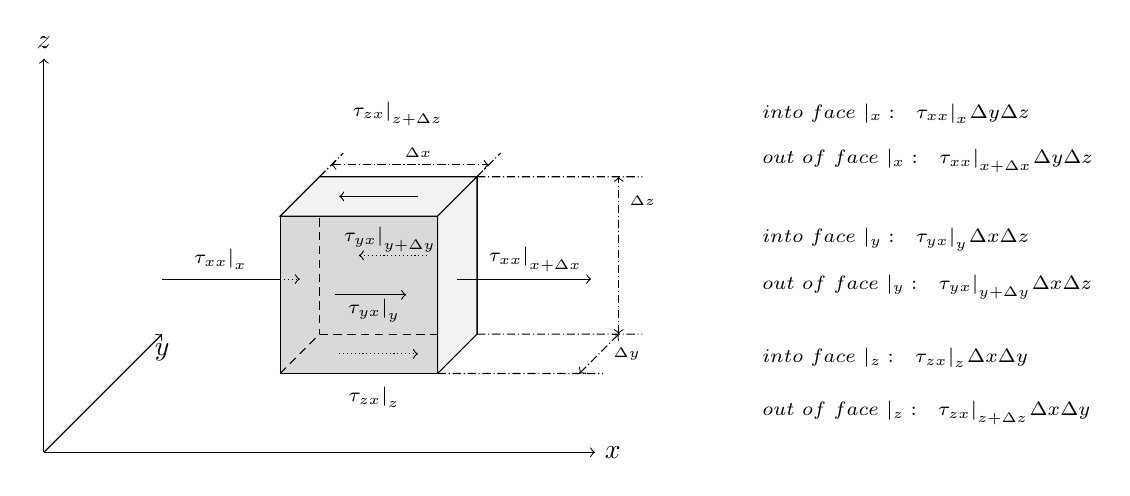
\begin{tikzpicture}
% Koordinatensystem
\draw[->] (0,0) -- (7,0) node[right] {$x$} coordinate(x axis);
\draw[->] (0,0) -- (0,5) node[above] {$z$} coordinate(y axis);
\draw[->] (0,0) -- (1.5,1.5) node[below] {$y$} coordinate(z axis);

% Quader
\draw [fill=gray!30] (3,1) -- (5,1) -- (5,3) -- (3,3) -- (3,1) ;

\draw [densely dashed] (3.5,1.5) -- (5.5,1.5);
\draw [] (5.5,1.5) -- (5.5,3.5) -- (3.5,3.5);
\draw [densely dashed] (3.5,3.5) -- (3.5,1.5);

\draw  [densely dashed] (3,1) -- (3.5,1.5);
\draw  [fill=gray!10] (5,1) -- (5.5,1.5) -- (5.5,3.5) -- (5,3) -- (5,1);
\draw  [fill=gray!10] (5,3) -- (5.5,3.5) --  (3.5,3.5) -- (3,3) -- (5,3);

%\draw (3,1) -- (3.5,3.5);
%\draw (3,3) -- (3.5,1.5);

% Pfeile
% rechts nach links
\draw [densely dotted, ->] (3,2.2) -- (3.25,2.2);


\draw [] (1.5,2.2) -- (3,2.2);

\draw [->] (5.25,2.2) -- (6.95,2.2);


% unten und oben
\draw [densely dotted, ->] (3.75,1.25) -- (4.75,1.25);
%\draw [-] (4.25,0.25) -- (4.25,1);
\draw [->] (4.75,3.25) -- (3.75,3.25);

% vorn und hinten
\draw [->] (3.7,2) -- (4.6,2);
\draw [densely dotted, <-] (4.0,2.5) -- (4.9,2.5);


% Punkte für Gleichungen
\node at (2.25,2.45) {\scriptsize $\tau_{xx}|_{_x}$};
\node at (6.25,2.45) {\scriptsize $\tau_{xx}|_{_{x+\Delta x}}$};

\node at (4.2,0.7) {\scriptsize $\tau_{zx}|_{_z}$};
\node at (4.5,4.3) {\scriptsize $\tau_{zx}|_{_{z+\Delta z}}$};

\node at (4.4,2.7) {\scriptsize $\tau_{yx}|_{_{y+\Delta y}}$};
\node at (4.2,1.8) {\scriptsize $\tau_{yx}|_{_y}$};



% Linien für dx dy dz
\draw [densely dashdotted] (5,1) -- (7.1,1)
	 (5.5,1.5) -- (7.6,1.5)
	 (5.5,3.5) -- (7.6, 3.5)
	 (3.5,3.5) -- (3.8,3.8)
	 (5.5,3.5) -- (5.8,3.8);

\draw [<->,densely dashdotted] (6.8,1) -- (7.3,1.5);
\node at (7.4,1.25) {\tiny $\Delta y$};

\draw [<->,densely dashdotted] (7.3,1.5) -- (7.3,3.5);
\node at (7.6,3.2) {\tiny $\Delta z$};

\draw [<->,densely dashdotted] (3.65,3.65) -- (5.65,3.65);
\node at (4.75,3.8) {\tiny $\Delta x$};

% Volumenpunkt
%\node at (4.25,2.25) {\tiny $\bullet$};
%\node at (4.5,2.25) {\tiny d$V$};



\node at (9,4.3) 	[right] {\scriptsize $\rmm{into~face~}|_x:~ ~ \tau_{xx}|_{_x} \Delta y \Delta z$};
\node at (9.0,3.7) 	[right] {\scriptsize $\rmm{out~of~face~}|_x:~ ~ \tau_{xx}|_{_{x + \Delta x}} \Delta y \Delta z$};

\node at (9,2.7) 	[right] {\scriptsize $\rmm{into~face~}|_y:~ ~ \tau_{yx}|_{_y} \Delta x \Delta z$};
\node at (9,2.1) 	[right] {\scriptsize $\rmm{out~of~face~}|_y:~ ~ \tau_{yx}|_{_{y + \Delta y}} \Delta x \Delta z$};

\node at (9,1.2) 	[right] {\scriptsize $\rmm{into~face~}|_z:~ ~ \tau_{zx}|_{_z} \Delta x \Delta y$};
\node at (9,0.5) 	[right] {\scriptsize $\rmm{out~of~face~}|_z:~ ~ \tau_{zx}|_{_{z + \Delta z}} \Delta x \Delta y$};
%
%
%
%
\end{tikzpicture}
\caption{Molecular transport of the momentum in $x$-direction in an arbitrary small volume element d$V$.}
\label{Abb_Grundlagen_2_Impulserhaltung}
\end{figure}
%
%

	Other phenomena that change the momentum inside the volume are given as
    a sum of forces. For example, we could have the gravitational acceleration
    and the pressure force acting on the volume.

    On the right side of figure \ref{Abb_Grundlagen_2_Impulserhaltung}, the
    terms that transport the $x$-component of the momentum through the
    surfaces by the molecular transport effect are given.
%
%
\subsubsection{Convection of the Momentum in $x$-Direction}
%
%
%
    The $x$-component of the momentum is transported by convection into the
    volume element through all six faces. Therefore, the convection of the
    momentum can be derived similarly to the convective transport of the mass.
    However, now we have to take care of the \textbf{vector} quantity.
    Thus, the momentum in the $x$-direction enters the volume at the
    face $|_{_x}$ and leaves the volume through the face $|_{_{x+\Delta x}}$;
    identical to the continuity equation. Nevertheless, it is also possible
    that the $x$-component of the momentum is transported through the faces in
    $y$- and $z$-direction (molecular transport). Hence, we can write the
    transport of the momentum due to convection; it is merely the velocity
    in $x$-direction multiplied by the \textbf{flux} through the face we are
    looking at (Newton's second law):
%
%
\begin{align*}
 \rmm{into~face~}&|_{_x}: ~~~~~~~
 (\rho u_x)u_x|_{_x} ~, \\
 \rmm{out~of~face~}&|_{_{x+\Delta x}}: ~~~
 (\rho u_x)u_x |_{_{x+\Delta x}} ~,
 \\
 \rmm{into~face~}&|_{_y} : ~~~~~~~
 (\rho u_y)u_x |_{_y} ~, \\
 \rmm{out~of~face~}&|_{_{y+\Delta y}} : ~~~
 (\rho u_y)u_x |_{_{y+\Delta y}} ~,
 \\
 \rmm{into~face~}&|_{_z} : ~~~~~~~
 (\rho u_z)u_x |_{_z} ~, \\
 \rmm{out~of~face~}&|_{_{z+\Delta z}} : ~~~
 (\rho u_z)u_x |_{_{z+\Delta z}} ~.
\end{align*}
%
%
	After combining the terms and using the face areas, we get:
%
%
\begin{align*}
  &\left(
    (\rho u_x)u_x |_{_x} - (\rho u_x)u_x |_{_{x+\Delta x}}
  \right)
  \Delta y \Delta z \\
  +&\left(
    (\rho u_y)u_x |_{_y} - (\rho u_y)u_x |_{_{y+\Delta y}}
  \right)
  \Delta x \Delta z  \\
  +&\left(
    (\rho u_z)u_x |_{_z} - (\rho u_z)u_x |_{_{z+\Delta z}}
  \right)
  \Delta x \Delta y ~.
\end{align*}
%
%
%
%
\subsubsection{Molecular Transport of the Momentum in $x$-Direction}
%
%
%
%
	Additionally, the $x$-component of the momentum is transported due to
    the molecular effects as demonstrated in figure
    \ref{Abb_Grundlagen_2_Impulserhaltung}. The effect is based on velocity
    differences (velocity gradients). As we can see in figure
    \ref{Abb_Grundlagen_2_Impulserhaltung}, different terms occur which include
    either the normal component $\tau_{xx}$ or the tangential component
    $\tau_{yx}$ or $\tau_{zx}$. Therefore, the molecular transport of the
    $x$-momentum through the surfaces can be written as:
%
%
\begin{align*}
  &\left(
    \tau_{xx} |_{_x} - \tau_{xx} |_{_{x+\Delta x}}
  \right)
  \Delta y \Delta z \\
  +&\left(
    \tau_{yx} |_{_y} - \tau_{yx} |_{_{y+\Delta y}}
  \right)
  \Delta x \Delta z \\
  +&\left(
    \tau_{zx} |_{_z} - \tau_{zx} |_{_{z+\Delta z}}
  \right)
  \Delta x \Delta y ~.
\end{align*}
%
%
      These terms represent additional fluxes of momentum through the surface.
      We consider these fluxes as stresses. $\tau_{xx}$ denotes the stress
      perpendicular to the direction we are looking at
      (here $\rmm{face}~|_{_x}$ and $\rmm{face}~|_{_{x+\Delta x}}$) and
      $\tau_{yx}$, $\tau_{zx}$ denote the $x$-directed tangential stresses
      which act on the faces with respect to the indices. All these stresses
      are known as shear stresses since they are generated concerning velocity
      gradients that introduce shearing.
%
%
%
%
\subsubsection{Additional Forces that Influence the Momentum}
%
%
%
      In most scientific and engineering tasks, the most essential forces that
      influence the momentum are the pressure and gravity force. The pressure
      force acts on the surface of the volume element while the gravitational
      force acts on the volume directly. Hence, we can derive the change of
      the $x$-momentum based on the pressure and gravitational force as follows:
%
%
\begin{equation*}
  \left(
    p|_{_x} - p|_{_{x+\Delta x}}
  \right)
  \Delta y \Delta z
+
  \rho g_x \Delta x \Delta y \Delta z ~.
\end{equation*}
%
%
%
%
\subsubsection{Conserved Momentum Equation}
%
%
      After we have all terms --- neglecting other influences such as surface
      tension and so on ---, the equation (\ref{EQUATION::momentum}) can be
      reconstructed with the corresponding mathematical expressions derived
      above. Of course, the accumulation of the momentum inside an arbitrary
      volume element is given by:
%
%
$$
 \frac{\Delta}{\Delta t} \rho u_x \Delta x \Delta y \Delta z ~.
$$
%
%
      Thus, for the momentum in $x$-direction we can write:
%
%
\begin{align*}
  \frac{\Delta}{\Delta t} \rho u_x \Delta x \Delta y \Delta z
=
  &\left(
  (\rho u_x)u_x|_{_x} - (\rho u_x)u_x|_{_{x+\Delta x}}
  \right) \Delta y \Delta z
 \\
  +&\left(
  (\rho u_y)u_x|_{_y} - (\rho u_y)u_x|_{_{y+\Delta y}}
  \right) \Delta x \Delta z
 \\
 +&\left(
  (\rho u_z)u_x|_{_z} - (\rho u_z)u_x|_{_{z+\Delta z}}
  \right) \Delta x \Delta y
 \\
 +&\left(
  \tau_{xx}|_{_x} - \tau_{xx}|_{_{x+\Delta x}}
  \right)\Delta y \Delta z
 \\
  +&\left(
  \tau_{yx}|_{_y} - \tau_{yx}|_{_{y+\Delta y}}
  \right) \Delta x \Delta z
 \\
  +&\left(
  \tau_{zx}|_{_z} - \tau_{zx}|_{_{z+\Delta z}}
  \right) \Delta x \Delta y
 \\
  +&\left(
  p|_{_x} - p|_{_{x+\Delta x}}
  \right) \Delta y \Delta z
 \\
  +&\rho g_x  \Delta x \Delta y \Delta z ~.
  \numberthis
\end{align*}
%
%
	Now, by dividing the whole equation by the volume d$V$, it follows:
%
%
\begin{align*}
   \frac{\Delta}{\Delta t} \rho u_x
&=
  \frac{(\rho u_x)u_x|_{_x} - (\rho u_x)u_x|_{_{x+\Delta x}}}{\Delta x}
+
  \frac{(\rho u_y)u_x|_{_y} - (\rho u_y)u_x|_{_{y+\Delta y}}}{\Delta y}
 \\
&+
  \frac{(\rho u_z)u_x|_{_z} - (\rho u_z)u_x|_{_{z+\Delta z}}}{\Delta z}
+
  \frac{\tau_{xx}|_{_x} - \tau_{xx}|_{_{x+\Delta x}}}{\Delta x}
+
  \frac{\tau_{yx}|_{_y} - \tau_{yx}|_{_{y+\Delta y}}}{\Delta y}
 \\
&+
  \frac{\tau_{zx}|_{_z} - \tau_{zx}|_{_{z+\Delta z}}}{\Delta z}
+
  \frac{p|_{_x} - p|_{_{x+\Delta x}}}{\Delta x}
+
  \rho g_x ~.
  \numberthis
\end{align*}
%
%
	Finally, we use the assumption of an infinitesimally small volume element
    (\ref{EQUATION::infty}) and time range (\ref{EQUATION::inftyTime}) to
    rewrite the $x$-component of the momentum equation. The $x$-component
    of the momentum is then written as:
%
%
\begin{equation}\boxed{\begin{aligned}
  \frac{\partial}{\partial t} \rho u_x
=
 &-\left(
      \frac{\partial}{\partial x} \rho u_x u_x
      +\frac{\partial}{\partial y} \rho u_y u_x
      +\frac{\partial}{\partial z} \rho u_z u_x
  \right)\\
 &-\left(
      \frac{\partial}{\partial x}  \tau_{xx}
      +\frac{\partial}{\partial y}  \tau_{yx}
      +\frac{\partial}{\partial z}  \tau_{zx}
  \right)
  -
  \frac{\partial p}{\partial x}
  +
  \rho g_x
  \label{EQUATION::momentumX}
\end{aligned}} ~.\end{equation}
%
%
    The other two space components are derived identically to the $x$-component.
    Thus, only the final formulation is given. For the $y$-component of the
    momentum, we get:
%
%
\begin{equation}\boxed{\begin{aligned}
  \frac{\partial}{\partial t} \rho u_y
=
 &-\left(
      \frac{\partial}{\partial x} \rho u_x u_y
      +\frac{\partial}{\partial y} \rho u_y u_y
      +\frac{\partial}{\partial z} \rho u_z u_y
  \right)\\
 &-\left(
      \frac{\partial}{\partial x}  \tau_{xy}
      +\frac{\partial}{\partial y}  \tau_{yy}
      +\frac{\partial}{\partial z}  \tau_{zy}
  \right)
  -
  \frac{\partial p}{\partial y}
  +
  \rho g_y
  \label{EQUATION::momentumY}
\end{aligned}}~,
\end{equation}
%
%
	and for the $z$-component we achieve:
%
%

\begin{equation}
\boxed{
\begin{aligned}
  \frac{\partial}{\partial t} \rho u_z
=
 &-\left(
      \frac{\partial}{\partial x} \rho u_x u_z
      +\frac{\partial}{\partial y} \rho u_y u_z
      +\frac{\partial}{\partial z} \rho u_z u_z
  \right)\\
 &-\left(
      \frac{\partial}{\partial x}  \tau_{xz}
      +\frac{\partial}{\partial y}  \tau_{yz}
      +\frac{\partial}{\partial z}  \tau_{zz}
  \right)
  -
  \frac{\partial p}{\partial z}
  +
  \rho g_z
  \label{EQUATION::momentumZ}
\end{aligned}
}~.
\end{equation}
%
%
	Introducing the gravitational acceleration vector \textbf{g}, the gradient
    of the pressure $  \nabla p$ and the shear-rate tensor $\boldsymbol \tau$
    that are defined as:
%
%
\begin{equation*}
    \nabla p
=
\left(
  \begin{matrix}
    \frac{\partial p}{\partial x} \\
    \frac{\partial p}{\partial y} \\
    \frac{\partial p}{\partial z} \\
  \end{matrix}
  \right),
  ~ ~ ~ ~ ~ ~ ~
\boldsymbol \tau
=
\left[
 \begin{matrix}
  \tau_{xx} ~~~~ \tau_{xy} ~~~~ \tau_{xz} \\
  \tau_{yx} ~~~~ \tau_{yy} ~~~~ \tau_{yz} \\
  \tau_{zx} ~~~~ \tau_{zy} ~~~~ \tau_{zz}
 \end{matrix}
\right],
  ~ ~ ~ ~ ~ ~ ~
\textbf{g}
=
\left(
 \begin{matrix}
  g_x \\
  g_y \\
  g_z
 \end{matrix}
\right),
\end{equation*}
%
%
	we can write the conserved momentum equation in vector form:
%
%
\begin{equation}
 \boxed{
    \frac{\partial}{\partial t} \rho \textbf{U}
=
    -   \nabla \bullet \left(\rho\textbf{U} \otimes \textbf{U}\right)
    -   \nabla \bullet \boldsymbol \tau
    -   \nabla p
    + \rho\textbf{g}
 }~.
 \label{EQUATION::momentumDiv}
\end{equation}
%
%
    \textbf{Note}, that the negative sign of the shear-rate tensor will change,
    if we introduce the definition of the shear-rate tensor $\boldsymbol \tau$
    later on.
%
%
%
%
%
\subsection{The Proof of the Transformation}
%
%
    The following section will investigate into the proof that equation
    (\ref{EQUATION::momentumDiv}) results in (\ref{EQUATION::momentumX}),
    (\ref{EQUATION::momentumY}) and (\ref{EQUATION::momentumZ}).
%
%
    For clearance, we will focus on each term separately. Starting with the
    first term, the time derivative, we get:
%
%
\begin{equation}
  \frac{\partial}{\partial t} \rho \textbf{U}
=
  \left(
  \begin{matrix}
      \frac{\partial}{\partial t} \rho u_x \\
      \frac{\partial}{\partial t} \rho u_y \\
      \frac{\partial}{\partial t} \rho u_z
  \end{matrix}
  \right)
\overset{!}{=}
\begin{cases}
  \frac{\partial}{\partial t} \rho u_x  ~~~ \rmm{of~}x-\rmm{momentum}\\
  \frac{\partial}{\partial t} \rho u_y  ~~~ \rmm{of~}y-\rmm{momentum}\\
  \frac{\partial}{\partial t} \rho u_z  ~~~ \rmm{of~}z-\rmm{momentum}
\end{cases} ~.
\end{equation}
%
%
    As we see, the time derivative term results in the same three terms that we
    have in the Cartesian formulation. The second term embraces the transport of
    momentum due to convection by the flux $\rho \textbf{U}$. To evaluate the
    term, we need the mathematics (\ref{EQUATION::dyadic}) and
    (\ref{EQUATION::divTensor}):
%
%
\begin{equation*}
 -   \nabla \bullet \left(\rho\textbf{U} \otimes \textbf{U}\right)
=
-   \nabla \bullet
  \left\{
  \rho
  \left(
  \begin{matrix}
    u_x \\
    u_y \\
    u_z
  \end{matrix}
  \right)
\otimes
\left(
  \begin{matrix}
    u_x \\
    u_y \\
    u_z
  \end{matrix}
  \right)
  \right\}
=
-   \nabla \bullet
  \left\{
  \rho
  \left[
  \begin{matrix}
    u_x u_x ~~~~ u_x u_y ~~~~ u_x u_z \\
    u_y u_x ~~~~ u_y u_y ~~~~ u_y u_z \\
    u_z u_x ~~~~ u_z u_y ~~~~ u_z u_z
  \end{matrix}
  \right]
  \right\}
\end{equation*}
%
%
%
\begin{equation*}
= -   \nabla \bullet
  \left[
  \begin{matrix}
    \rho u_x u_x ~~~~ \rho u_x u_y ~~~~ \rho u_x u_z \\
    \rho u_y u_x ~~~~ \rho u_y u_y ~~~~ \rho u_y u_z \\
    \rho u_z u_x ~~~~ \rho u_z u_y ~~~~ \rho u_z u_z
  \end{matrix}
  \right]
=
- \left(
  \begin{matrix}
    \frac{\partial}{\partial x} \\
    \frac{\partial}{\partial y} \\
    \frac{\partial}{\partial z}
  \end{matrix}
  \right)
  \bullet
  \left[
  \begin{matrix}
    \rho u_x u_x ~~~~ \rho u_x u_y ~~~~ \rho u_x u_z \\
    \rho u_y u_x ~~~~ \rho u_y u_y ~~~~ \rho u_y u_z \\
    \rho u_z u_x ~~~~ \rho u_z u_y ~~~~ \rho u_z u_z
  \end{matrix}
  \right]
\end{equation*}
%
%
\begin{equation*}
= - \left[
  \begin{matrix}
    \frac{\partial}{\partial x} \rho u_x u_x +
    \frac{\partial}{\partial y} \rho u_y u_x +
    \frac{\partial}{\partial z} \rho u_z u_x \\
    \frac{\partial}{\partial x} \rho u_x u_y +
    \frac{\partial}{\partial y} \rho u_y u_y +
    \frac{\partial}{\partial z} \rho u_z u_y \\
    \frac{\partial}{\partial x} \rho u_x u_z +
    \frac{\partial}{\partial y} \rho u_y u_z +
    \frac{\partial}{\partial z} \rho u_z u_z
  \end{matrix}
  \right]
\overset{!}{=}
\begin{cases}
  -\left(
      \frac{\partial}{\partial x} \rho u_x u_x
      +\frac{\partial}{\partial y} \rho u_y u_x
      +\frac{\partial}{\partial z} \rho u_z u_x
  \right)% ~~~ \rmm{of~}x- \rmm{mom.}\\
  \\
  -\left(
      \frac{\partial}{\partial x} \rho u_x u_y
      +\frac{\partial}{\partial y} \rho u_y u_y
      +\frac{\partial}{\partial z} \rho u_z u_y
  \right)% ~~~ \rmm{of~}y- \rmm{mom.}\\
  \\
  -\left(
      \frac{\partial}{\partial x} \rho u_x u_z
      +\frac{\partial}{\partial y} \rho u_y u_z
      +\frac{\partial}{\partial z} \rho u_z u_z
  \right)% ~~~ \rmm{of~}z- \rmm{mom.}
\end{cases}
  .
\end{equation*}
%
%
    Again, we can see that the terms are equal and we end up with the same set
    of equations. Now we investigate into the third term that describes shearing
    due to the gradients of the velocities.  Using the convention
    (\ref{EQUATION::divTensor}) for the shear-rate tensor $\boldsymbol \tau$, we
    get:
%
%
\begin{equation*}
  -  \nabla \bullet \boldsymbol \tau
=
  -  \nabla \bullet
  \left[
  \begin{matrix}
  \tau_{xx} ~~~~ \tau_{xy} ~~~~ \tau_{xz} \\
  \tau_{yx} ~~~~ \tau_{yy} ~~~~ \tau_{yz} \\
  \tau_{zx} ~~~~ \tau_{zy} ~~~~ \tau_{zz}
  \end{matrix}
  \right]
=
\end{equation*}
\begin{equation*}
- \left[
  \begin{matrix}
  \frac{\partial}{\partial x}\tau_{xx} + \frac{\partial}{\partial y} \tau_{yx} + \frac{\partial}{\partial z} \tau_{zx} \\
  \frac{\partial}{\partial x}\tau_{xy} + \frac{\partial}{\partial y} \tau_{yy} + \frac{\partial}{\partial z}\tau_{zy} \\
  \frac{\partial}{\partial x}\tau_{xz} + \frac{\partial}{\partial y} \tau_{yz} + \frac{\partial}{\partial z} \tau_{zz}
  \end{matrix}
  \right]
\overset{!}{=}
  \begin{cases}
  -\left(
      \frac{\partial}{\partial x}  \tau_{xx}
      +\frac{\partial}{\partial y}  \tau_{yx}
      +\frac{\partial}{\partial z}  \tau_{zx}
  \right) ~ \rmm{of~}x ~ \rmm{momentum} \\
  -\left(
      \frac{\partial}{\partial x}  \tau_{xy}
      +\frac{\partial}{\partial y}  \tau_{yy}
      +\frac{\partial}{\partial z}  \tau_{zy}
  \right) ~ \rmm{of~}y ~ \rmm{momentum} \\
    -\left(
      \frac{\partial}{\partial x}  \tau_{xz}
      +\frac{\partial}{\partial y}  \tau_{yz}
      +\frac{\partial}{\partial z}  \tau_{zz}
  \right) ~ \rmm{of~}z ~ \rmm{momentum}
  \end{cases}
  .
\end{equation*}
%
%
    At last the pressure and gravitational acceleration term are analyzed. For
    the pressure term we need the definition of equation
    (\ref{EQUATION::gradientScalar}) and for the gravitational term equation
    (\ref{EQUATION::simple}). It follows:
%
%
\begin{equation*}
  -  \nabla p
=
  -
  \left(
  \begin{matrix}
   \frac{\partial}{\partial x} \\
   \frac{\partial}{\partial y} \\
   \frac{\partial}{\partial z}
  \end{matrix}
  \right) p
=
-
  \left(
  \begin{matrix}
   \frac{\partial p}{\partial x} \\
   \frac{\partial p}{\partial y} \\
   \frac{\partial p}{\partial z}
  \end{matrix}
  \right)
\overset{!}{=}
  \begin{cases}
  -\frac{\partial p}{\partial x} ~ \rmm{of~}x ~ \rmm{momentum} \\
  -\frac{\partial p}{\partial y} ~ \rmm{of~}y ~ \rmm{momentum} \\
  -\frac{\partial p}{\partial z} ~ \rmm{of~}z ~ \rmm{momentum}
  \end{cases},
\end{equation*}
\begin{equation*}
  \rho \textbf{g}
=
  \rho
  \left(
  \begin{matrix}
    g_x \\
    g_y \\
    g_z
  \end{matrix}
  \right)
=
  \left(
  \begin{matrix}
    \rho g_x \\
    \rho g_y \\
    \rho g_z
  \end{matrix}
  \right)
\overset{!}{=}
  \begin{cases}
  \rho g_x ~ \rmm{of~}x ~ \rmm{momentum} \\
  \rho g_y ~ \rmm{of~}y ~ \rmm{momentum} \\
  \rho g_z ~ \rmm{of~}z ~ \rmm{momentum}
  \end{cases} .
\end{equation*}
%
%
	 As we \texttt{proofed} now, the vector form ends up in the Cartesian form.

     If we want to solve this equation now, it is necessary to know the
     shear-rate tensor $\boldsymbol \tau$. We are going to investigate into that
     quantity in chapter \ref{CHAPTER::shearrate}. Further representations of
     the momentum equation can be found in chapter
     \ref{CHAPTER::derivationsOfMomentum}. The implementation of the momentum
     equation in \OF will be discussed in chapter
     \ref{CHAPTER::ShearRateTensorFunctions}; especially the treatment of the
     diffusion term.  Keep in mind that equation (\ref{EQUATION::momentumDiv})
     includes \textit{only} the gravitational acceleration and pressure force.
     If there are further phenomena (forces) influencing the momentum equation,
     these terms have to be taken into account.
%
%
%
\subsection{Integral Form of the Conserved Momentum Equation}
%
%
    The integral form of the momentum equation (\ref{EQUATION::momentumDiv}) can
    be obtained by using the Gauss theorem (\ref{EQUATION::gausstheorem}). It
    follows:
%
%
%
\begin{equation}
 \boxed{
    \frac{\partial}{\partial t} \int \rho \textbf{U} \mathrm{d}V
=
    -   \oint (\rho\textbf{U} \otimes \textbf{U}) \cdot \textbf{n} \mathrm{d}S
    -   \oint \boldsymbol \tau  \cdot \textbf{n} \mathrm{d}S
    -   \oint p\textbf{I} \cdot \textbf{n} \mathrm{d}S
    + \int \rho\textbf{g}  \mathrm{d}V
 } ~.
\end{equation}
%
%
%
\subsection{Non-Conserved Momentum Equation}
%
%
    We can manipulate the conserved momentum equation with the continuity
    equation (\ref{EQUATION::massCompressible}). Hence, we get the
    non-conservative form. For that, we first consider equation
    (\ref{EQUATION::momentumDiv}) and split the time and convection term by
    using the product rule. The time derivative becomes:
%
%
\begin{equation}
  \frac{\partial}{\partial t} \rho \textbf{U}
=
  \rho \frac{\partial}{\partial t} \textbf{U} + \textbf{U} \frac{\partial}{\partial t} \rho ~,
\end{equation}
%
%
    and the convection term can be rewritten using equation
    (\ref{EQUATION::productRuleVV}). It follows:
%
%
\begin{equation}
  \nabla \bullet \left(\rho\textbf{U} \otimes \textbf{U}\right)
=
  \underbrace{\rho\textbf{U} \bullet \underbrace{\nabla \otimes \textbf{U}}_{\mathrm{gradient}}}_{\mathrm{inner~product}} + \textbf{U} \underbrace{\nabla \bullet (\rho\textbf{U})}_{\mathrm{divergence}} ~.
\end{equation}
%
%
    Replacing these terms into equation (\ref{EQUATION::momentumDiv}) and put
    the convection terms to the LHS, we end up with:
%
%
\begin{equation}
   \rho \frac{\partial}{\partial t} \textbf{U} + \textbf{U} \frac{\partial}{\partial t} \rho
+
   \rho\textbf{U} \bullet \nabla \otimes \textbf{U} + \textbf{U} \nabla \bullet (\rho\textbf{U})
=
   .~.~.
\end{equation}
%
%
    After analyzing the equation, we see that we can take out $\rho$ and
    $\textbf{U}$:
%
%
\begin{equation}
   \rho \left[\frac{\partial}{\partial t} \textbf{U} + \textbf{U} \bullet \nabla \otimes \textbf{U}\right]
+
\textbf{U} \underbrace{\left[\cancel{\frac{\partial}{\partial t} \rho + \nabla \bullet (\rho\textbf{U})}\right]}_{\mathrm{continuity}}
=
   .~.~.
\end{equation}
%
%
    It is clear that the second term is zero due to the continuity equation.
    Applying the definition of the total derivative
    (\ref{EQUATION::totalDerivative}), we can write the non-conservative form of
    the momentum equation as:
%
%
\begin{equation}
  \rho \frac{\mathrm{D}\textbf{U}}{\mathrm{D}t}
=
    -   \nabla \bullet \boldsymbol \tau
    -   \nabla p
    + \rho\textbf{g}
\label{EQUATION::momentumDivNon}
\end{equation}
%
%
    \textbf{Remark}: As already mentioned before, the negative sign of the first
    term on the RHS will vanish after we introduced the definition of the
    shear-rate components $\tau_{ii}$.
%
%
%
%
%

%==============================================================================
\end{document}
%==============================================================================
